The correctness of the algorithm follows by induction over the construction:
If the correct co-routine stops in the end state for all possible
constructions of the Thompson construction under the assumption that simpler
automata do the same, it follows that no matter how complex the automata get,
the algorithm will have the correct output.

The proof will be in three steps:
\begin{description}
  \item[Foundation] Firstly we will show that a simple path
    will get the correct indices, i.e. that the indexing of the capture works correctly.
  \item[Induction] Secondly we will show that an automaton constructed from
    correct sub-automata is correct.
  \item[Exhaustion] Thirdly and lastly we will show that every construction
    of the automata satisfies the induction property and thus that every
    automaton created by the modified Thompson construction is executed correctly.
\end{description}

\begin{defn}
  A NFA $A$ is \emph{well-formed} if there is a regular expression $r$ that
  will be compiled to $A$ via the execution of algorithm~\ref{TODO(modified thompson}.

  Specifically this means that opening and closing of groups happens in
  correct order and that there is no path avoiding the closing of the group
  in case the opening is passed. Further a well-formed automaton can be
  deconstructed into subautomata corresponding to the Thompson construction.
\end{defn}

\begin{defn}
  A NFA $A$ is a \emph{chain} of subautomatons
  $A_1\rightarrow A_2 \rightarrow \dots \rightarrow A_m$ if it is well-formed
  and the picture
  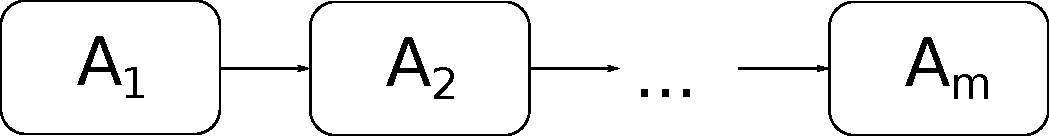
\includegraphics[width=0.8\linewidth]{graphs/chain}

  holds, i.e. the automatons $A_i$ appear in order and there are only 
  $\varepsilon$-transitions forward.
\end{defn}

\begin{lemma}
  Let $A$ be a well-formed NFA in which each state contains only one outgoing edge (or
  zero in the case of the end state) described by
  $a_1\xrightarrow_{t_1}\dots\xrightarrow_{t_{m}}\mathtt{a_{m+1}}$. Let further
  $s=\"s_1\dots s_n\"$ be a string to be matched by $A$, then the coroutine in
  $a_{m+1}$ after reading $s$ will be
\end{lemma}
